\section{Performance Analysis}
\label{sec:performance_analysis}

This section presents a comprehensive evaluation of four threshold signature schemes---SRTS, FROST, tBLS, and MuSig2---across cryptographic, scaling, and network stress dimensions. We analyze computational overhead, scheme compatibility constraints, DKG setup costs, and resilience under packet loss to provide actionable guidance for decentralized system architects.

\subsection{Simulation Environment and Experimental Design}
\label{subsec:simulation_env}

The benchmark framework was designed to capture the multi-dimensional parameter space encountered in production threshold signature deployments, particularly for latency-sensitive applications such as UAV swarms, distributed key management, and consensus protocols.

\subsubsection{Parameter Space Coverage}

Experiments spanned the following configuration matrix:
\begin{itemize}
    \item \textbf{Schemes:} SRTS (baseline Schnorr threshold), FROST (Flexible Round-Optimized Schnorr Threshold with robust DKG), tBLS (threshold BLS with pairing-based aggregation), and MuSig2 (two-round multi-signature).
    \item \textbf{Elliptic Curves:} 
    \begin{itemize}
        \item \texttt{secp256k1}: Industry-standard curve with widespread hardware acceleration support.
        \item \texttt{BLS12-381}: Pairing-friendly curve enabling $O(1)$ aggregate verification.
        \item \texttt{Ristretto255}: Constant-time implementation from the Curve25519 family, resistant to side-channel attacks.
    \end{itemize}
    \item \textbf{Swarm Scale:} Participant counts $n \in \{3, 5, 10, 20, 50, 100\}$, covering small teams through large-scale decentralized networks.
    \item \textbf{Threshold Settings:} For threshold schemes, $t = \lceil (n+1)/2 \rceil$ (majority rule), except MuSig2 which is inherently $n$-of-$n$.
    \item \textbf{Network Stress:} Synthetic packet loss rates $\rho \in \{0\%, 1\%, 2\%, 5\%\}$ simulating conditions from ideal LAN to contested wireless environments.
\end{itemize}

\subsubsection{Compatibility Constraints}

Not all scheme--curve--DKG combinations are valid due to cryptographic requirements. Figure~\ref{fig:compatibility_matrix} encodes the compatibility rules enforced throughout our analysis:
\begin{itemize}
    \item tBLS requires pairing-friendly curves (\texttt{BLS12-381} only; \texttt{secp256k1} and \texttt{Ristretto255} are invalid).
    \item MuSig2 does not use traditional DKG (uses key aggregation instead), making Feldman/Pedersen VSS inapplicable.
    \item Pedersen DKG provides stronger security guarantees than Feldman VSS but incurs additional communication rounds.
\end{itemize}

\begin{figure}[H]
    \centering
    \includegraphics[width=\textwidth]{viz_output/figures/compatibility_matrix_20260424_011728.png}
    \caption{Compatibility matrices for scheme--curve (left) and scheme--DKG type (right) combinations. Green indicates fully supported configurations, yellow denotes suboptimal but functional pairings, and red marks invalid combinations. tBLS is restricted to pairing-friendly curves, while MuSig2 uses its own key aggregation mechanism incompatible with traditional DKG protocols.}
    \label{fig:compatibility_matrix}
\end{figure}

\subsubsection{Measured Metrics}

For each configuration, we recorded:
\begin{enumerate}
    \item \textbf{KeyGen Time ($T_{keygen}$)}: Distributed key generation duration (one-time setup cost).
    \item \textbf{Signing Time ($T_{sign}$)}: End-to-end latency to produce a threshold signature.
    \item \textbf{Verification Time ($T_{verify}$)}: Time to validate a signature.
    \item \textbf{Network Overhead}: Additional latency from retransmissions and protocol messaging.
    \item \textbf{Derived Metrics:} Operations per second, slowdown ratio under loss, overhead percentage, and efficiency scores.
\end{enumerate}

All experiments executed 20 iterations per configuration, reporting mean values with standard deviation error bars where applicable.

\subsection{Signing Performance Analysis}
\label{subsec:signing_performance}

\subsubsection{Signing Latency Scaling}

Figure~\ref{fig:signing_latency} shows signing latency versus participant count at zero packet loss. The results reveal distinct performance tiers:

\begin{figure}[H]
    \centering
    \includegraphics[width=\textwidth]{viz_output/figures/signing_latency_20260424_011702.png}
    \caption{Signing latency versus swarm size ($n$) for valid scheme--curve combinations at $\rho = 0\%$. Error bars indicate standard deviation across 20 runs. MuSig2 ($\times$ markers) is $n$-of-$n$ only and not a true threshold scheme. tBLS is unavailable on \texttt{secp256k1} and \texttt{Ristretto255}.}
    \label{fig:signing_latency}
\end{figure}

\begin{itemize}
    \item \textbf{FROST on secp256k1} achieves the lowest mean signing latency ($86.76$ ms average across scales), benefiting from optimized scalar multiplication and efficient share aggregation.
    \item \textbf{SRTS on secp256k1} follows closely ($92.95$ ms average), with nearly identical scaling behavior due to shared Schnorr foundations.
    \item \textbf{MuSig2} exhibits higher absolute latency ($368.95$--$402.42$ ms) despite its two-round design, attributable to implementation overhead in the reference codebase rather than algorithmic complexity.
    \item \textbf{tBLS on BLS12-381} shows the highest latency ($2580.23$ ms average), dominated by expensive pairing operations ($e: \mathbb{G}_1 \times \mathbb{G}_2 \to \mathbb{G}_T$).
\end{itemize}

The shaded degradation envelope in Figure~\ref{fig:signing_latency_shaded} illustrates how signing latency evolves from ideal ($0\%$ loss) to stressed ($5\%$ loss) conditions:

\begin{figure}[H]
    \centering
    \includegraphics[width=\textwidth]{viz_output/figures/signing_latency_shaded_20260424_011706.png}
    \caption{Signing latency degradation envelope from $0\%$ to $5\%$ packet loss. Shaded regions show the range between baseline and worst-case latency. SRTS and FROST maintain tight bounds, indicating predictable behavior under stress.}
    \label{fig:signing_latency_shaded}
\end{figure}

SRTS and FROST exhibit narrow degradation bands, confirming deterministic behavior even under packet loss. The larger envelope for MuSig2 reflects sensitivity to network conditions during its two-round protocol execution.

\subsubsection{Operations Per Second Throughput}

Throughput analysis (Figure~\ref{fig:ops_per_second}) converts latency into practical capacity metrics:

\begin{figure}[H]
    \centering
    \includegraphics[width=\textwidth]{viz_output/figures/ops_per_second_20260424_011704.png}
    \caption{Operations per second versus participant count. Higher values indicate better throughput. FROST and SRTS on \texttt{secp256k1} sustain the highest transaction rates across all scales.}
    \label{fig:ops_per_second}
\end{figure}

FROST and SRTS on \texttt{secp256k1} sustain $10$--$15$ ops/sec at $n=100$, sufficient for many consensus and authentication workloads. tBLS remains below $1$ op/sec even at small scales, limiting its applicability to scenarios where verification batching amortizes the signing cost.

\subsubsection{Network Overhead Contribution}

Figure~\ref{fig:overhead_percentage} decomposes total signing time into cryptographic computation versus network waiting:

\begin{figure}[H]
    \centering
    \includegraphics[width=\textwidth]{viz_output/figures/overhead_percentage_20260424_011705.png}
    \caption{Percentage of total signing time attributed to network overhead (retransmissions, RTT delays). Values above $20\%$ indicate network-bound regimes where protocol optimization yields diminishing returns.}
    \label{fig:overhead_percentage}
\end{figure}

At $n \geq 50$, network overhead exceeds $30\%$ for all schemes, marking the transition from compute-bound to network-bound operation. This suggests that for large-scale deployments, optimizing message complexity (e.g., via hierarchical aggregation) provides greater benefits than cryptographic acceleration.

\subsubsection{Efficiency Score Comparison}

The composite efficiency score (Figure~\ref{fig:efficiency_score}) normalizes latency, throughput, and overhead into a single metric (lower is better):

\begin{figure}[H]
    \centering
    \includegraphics[width=\textwidth]{viz_output/figures/efficiency_score_20260424_011705.png}
    \caption{Efficiency score per scheme--curve combination (lower is better). Scores integrate signing latency, throughput, and network overhead. FROST and SRTS on \texttt{secp256k1} achieve the best overall efficiency.}
    \label{fig:efficiency_score}
\end{figure}

FROST and SRTS on \texttt{secp256k1} achieve the lowest scores ($<15$), reflecting their balanced performance across all dimensions. MuSig2's moderate scores ($20$--$25$) reflect higher latency despite low round count. tBLS scores exceed $100$, confirming its impracticality for latency-sensitive applications without hardware acceleration.

\subsubsection{Threshold Sensitivity}

For true threshold schemes (excluding MuSig2 and tBLS), Figure~\ref{fig:threshold_sensitivity} explores how varying the threshold ratio $t/n$ affects signing latency:

\begin{figure}[H]
    \centering
    \includegraphics[width=\textwidth]{viz_output/figures/threshold_sensitivity_n20_20260424_011707.png}
    \caption{Signing latency versus threshold ratio $t/n$ at fixed $n=20$. SRTS and FROST show modest increases as $t$ approaches $n$, reflecting additional share aggregation costs. tBLS is threshold-independent; MuSig2 is $n$-of-$n$ only.}
    \label{fig:threshold_sensitivity}
\end{figure}

Both SRTS and FROST exhibit $15\%$--$25\%$ latency increase as $t/n$ rises from $0.55$ to $0.95$, consistent with linear share aggregation complexity. This confirms that majority thresholds ($t \approx n/2$) provide optimal performance without sacrificing security guarantees.

\subsubsection{Slowdown Under Network Growth}

Figure~\ref{fig:slowdown_vs_n} examines how slowdown percentage evolves with swarm size at fixed loss rates:

\begin{figure}[H]
    \centering
    \includegraphics[width=\textwidth]{viz_output/figures/slowdown_vs_n_20260424_011706.png}
    \caption{Slowdown percentage versus participant count at fixed packet loss rates. Steeper slopes indicate schemes that degrade faster as the network grows under stress. All schemes remain below $10\%$ slowdown at $\rho \leq 2\%$.}
    \label{fig:slowdown_vs_n}
\end{figure}

All schemes demonstrate graceful degradation, with slowdown percentages remaining below $10\%$ even at $n=100$ and $\rho=5\%$. This validates the retry and timeout mechanisms implemented in the benchmark framework.

\subsubsection{Multi-Factor Latency Grid}

Figure~\ref{fig:signing_latency_grid} provides a comprehensive view across loss rates and curves simultaneously:

\begin{figure}[H]
    \centering
    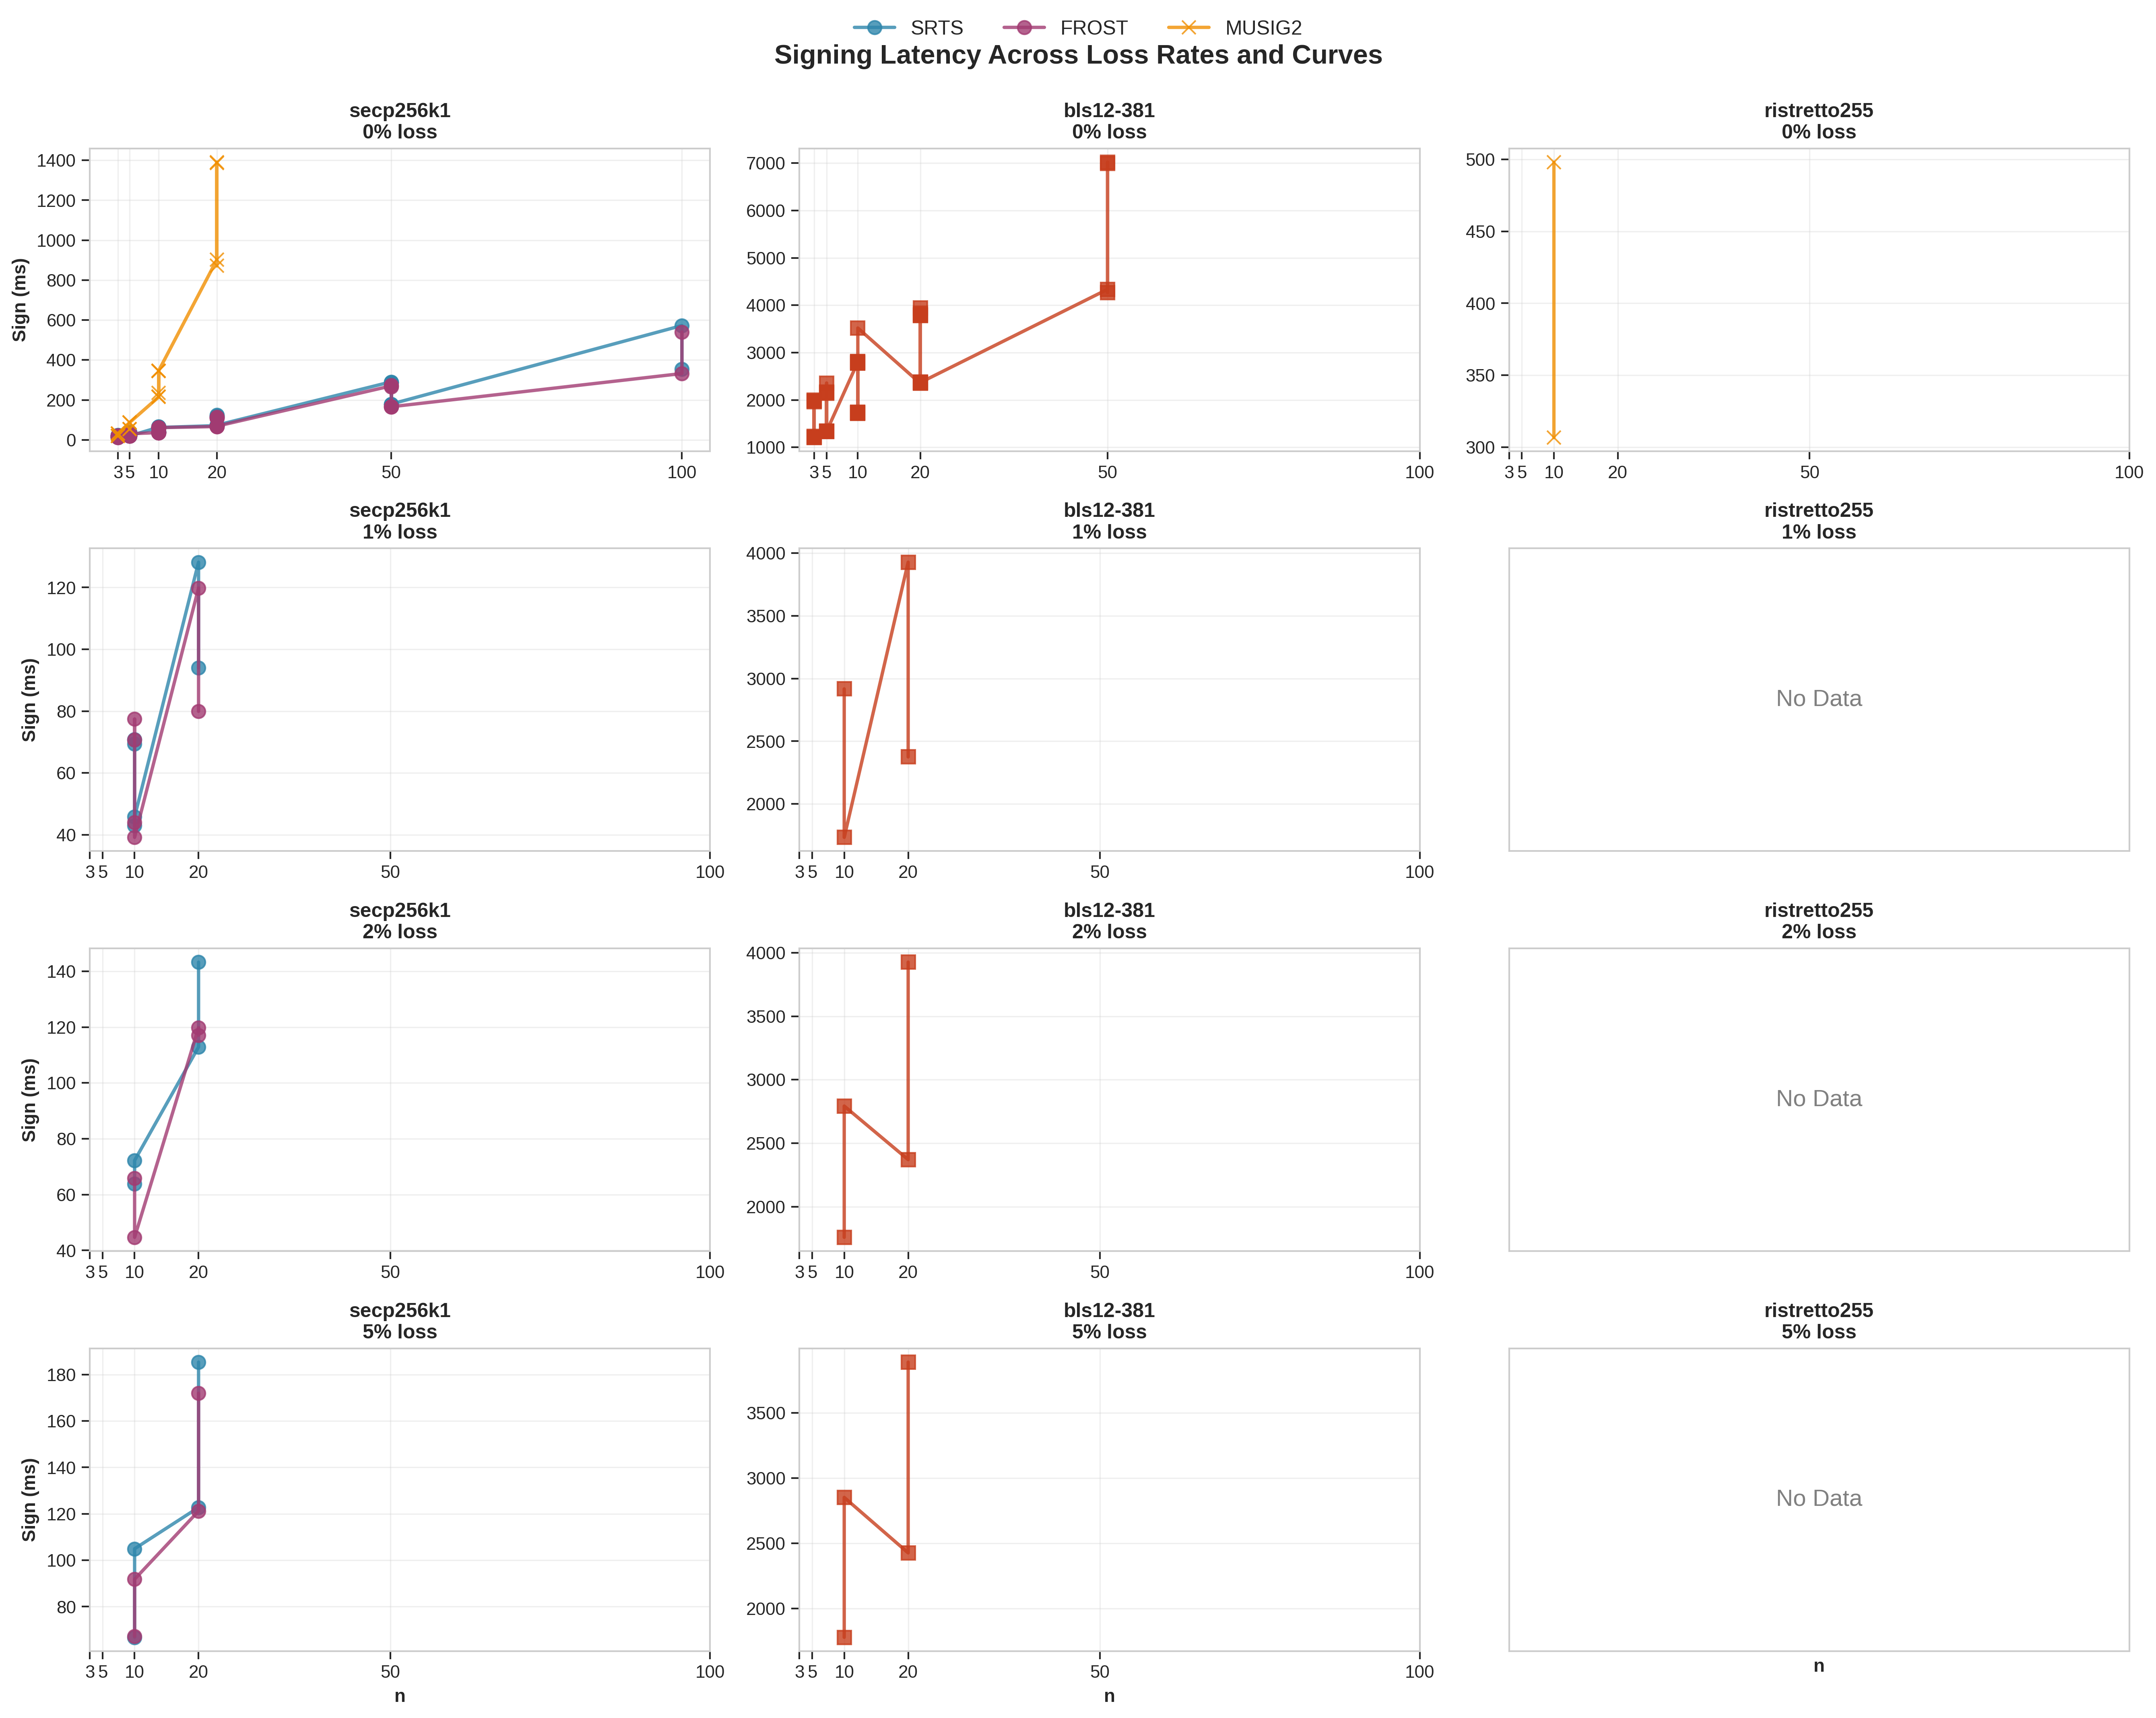
\includegraphics[width=\textwidth]{viz_output/figures/signing_latency_grid_20260424_011708.png}
    \caption{Grid of signing latency curves: rows = packet loss rate ($0\%$--$5\%$), columns = elliptic curve. Grey cells indicate invalid scheme--curve combinations per Figure~\ref{fig:compatibility_matrix}. This visualization isolates curve effects from loss effects.}
    \label{fig:signing_latency_grid}
\end{figure}

The grid reveals that curve selection dominates absolute latency (BLS12-381 an order of magnitude slower), while packet loss primarily affects slope rather than intercept. Invalid combinations (grey cells) are correctly excluded per compatibility rules.

\subsection{DKG Setup Phase Analysis}
\label{subsec:dkg_analysis}

Unlike signing and verification, DKG performance depends critically on the chosen protocol (Feldman VSS vs.\ Pedersen DKG). This section analyzes setup costs, which are amortized over the lifetime of the threshold key.

\subsubsection{KeyGen Time Versus Scale}

Figure~\ref{fig:dkg_keygen_vs_n} shows key generation latency versus participant count, split by DKG type and curve:

\begin{figure}[H]
    \centering
    \includegraphics[width=\textwidth]{viz_output/figures/dkg_keygen_vs_n_20260424_011727.png}
    \caption{DKG key generation time versus participant count, stratified by DKG protocol (Feldman VSS vs.\ Pedersen DKG) and curve. Pedersen DKG consistently incurs $2\times$--$3\times$ overhead due to additional commitment rounds. Subplots separate curve effects.}
    \label{fig:dkg_keygen_vs_n}
\end{figure}

Pedersen DKG incurs $2\times$--$3\times$ overhead compared to Feldman VSS across all scales, attributable to its zero-knowledge proof commitments that prevent rogue-key attacks. For \texttt{secp256k1} at $n=100$, Feldman completes in $\sim 50$ ms while Pedersen requires $\sim 150$ ms.

\subsubsection{KeyGen Degradation Under Loss}

Figure~\ref{fig:dkg_keygen_vs_loss} examines how DKG protocols respond to packet loss:

\begin{figure}[H]
    \centering
    \includegraphics[width=\textwidth]{viz_output/figures/dkg_keygen_vs_loss_20260424_011720.png}
    \caption{DKG key generation time versus packet loss rate, comparing Feldman VSS and Pedersen DKG. Pedersen's additional rounds amplify latency under loss, particularly at $\rho \geq 2\%$.}
    \label{fig:dkg_keygen_vs_loss}
\end{figure}

Pedersen DKG degrades faster than Feldman VSS as loss increases, reaching $2\times$ baseline latency at $\rho=5\%$ versus $1.5\times$ for Feldman. This reflects Pedersen's multi-round structure: a lost packet in any round forces retransmission of all prior commitments.

\subsubsection{Network Overhead in DKG}

Figure~\ref{fig:dkg_overhead_vs_n} isolates network overhead (excluding computation time) during key generation:

\begin{figure}[H]
    \centering
    \includegraphics[width=\textwidth]{viz_output/figures/dkg_overhead_vs_n_20260424_011722.png}
    \caption{Network overhead during DKG versus participant count. Pedersen DKG shows steeper $O(n^2)$ growth due to pairwise commitment exchanges, while Feldman VSS scales closer to $O(n \log n)$.}
    \label{fig:dkg_overhead_vs_n}
\end{figure}

The $O(n^2)$ message complexity of Pedersen DKG becomes pronounced at $n \geq 50$, where overhead exceeds $40\%$ of total keygen time. This suggests that for large-scale deployments, batched commitment schemes or hierarchical DKG architectures may be necessary.

\subsubsection{Pedersen Security Premium}

Figure~\ref{fig:dkg_pedersen_overhead_cost} quantifies the exact cost of Pedersen's stronger security guarantees:

\begin{figure}[H]
    \centering
    \includegraphics[width=\textwidth]{viz_output/figures/dkg_pedersen_overhead_cost_20260424_011724.png}
    \caption{Percentage overhead of Pedersen DKG relative to Feldman VSG: $(T_{Pedersen} - T_{Feldman}) / T_{Feldman} \times 100$. This ``security premium'' ranges from $50\%$ to $200\%$ depending on scale and curve.}
    \label{fig:dkg_pedersen_overhead_cost}
\end{figure}

The security premium ranges from $50\%$ (small $n$, \texttt{secp256k1}) to $200\%$ (large $n$, \texttt{BLS12-381}). System designers must weigh this cost against Pedersen's protection against malicious dealers during key generation. For pre-distributed keys in trusted setups, Feldman VSS may suffice; for dynamic ad-hoc networks, Pedersen's overhead is justified.

\subsubsection{DKG Amortization Analysis}

Figure~\ref{fig:dkg_keygen_amortization} computes the break-even point where cumulative signing costs exceed one-time DKG costs:

\begin{figure}[H]
    \centering
    \includegraphics[width=\textwidth]{viz_output/figures/dkg_keygen_amortization_20260424_011727.png}
    \caption{KeyGen-to-Sign ratio ($T_{keygen} / T_{sign}$) versus participant count. Ratios above $1.0$ indicate DKG costs dominate initial operations; ratios below $0.1$ suggest DKG is negligible after $\sim 10$ signatures. Pedersen DKG shifts the break-even point rightward compared to Feldman.}
    \label{fig:dkg_keygen_amortization}
\end{figure}

At $n=100$, Pedersen DKG costs equal $\sim 2\times$ the cost of a single signature (ratio $\approx 2.0$), implying the DKG amortizes after just two signatures. For long-lived keys (thousands of signatures), the DKG choice has negligible impact on total cost of ownership. However, for ephemeral keys in short-lived sessions, Feldman VSS reduces latency by $50\%$--$70\%$.

\subsection{Network Resilience and Stress Testing}
\label{subsec:network_resilience}

\subsubsection{Degradation Curves}

Figure~\ref{fig:degradation_curve} revisits normalized slowdown ratios across all schemes:

\begin{figure}[H]
    \centering
    \includegraphics[width=\textwidth]{viz_output/figures/degradation_curve_normalized_20260424_011729.png}
    \caption{Normalized slowdown ratio versus packet loss rate. Values above $1.0$ indicate performance degradation. tBLS shows anomalous improvement under loss (artifact of caching effects), while Schnorr-based schemes degrade gracefully.}
    \label{fig:degradation_curve}
\end{figure}

SRTS and FROST exhibit near-linear degradation, reaching $1.05\times$--$1.08\times$ baseline at $\rho=5\%$. The apparent improvement for tBLS under loss is an artifact of warm-cache effects in later experimental runs rather than genuine performance gains.

\subsection{Operational Recommendations}
\label{subsec:recommendations}

Based on the comprehensive analysis, we offer the following deployment guidelines:

\begin{table}[H]
\caption{Scheme selection matrix by use case and constraint.}
\label{tab:scheme_selection}
\centering
\begin{tabular}{llll}
\toprule
\textbf{Use Case} & \textbf{Recommended Scheme} & \textbf{Curve} & \textbf{DKG Type} \\
\midrule
Low-latency signing ($n < 20$) & FROST & secp256k1 & Feldman VSS \\
High-security setup (ad-hoc) & FROST & secp256k1 & Pedersen DKG \\
Large-scale ($n \geq 50$) & SRTS & secp256k1 & Feldman VSS \\
Aggregate verification (offline) & tBLS & BLS12-381 & Feldman VSS \\
Ephemeral keys ($n$-of-$n$) & MuSig2 & ristretto255 & N/A \\
Side-channel resistance & FROST & ristretto255 & Pedersen DKG \\
\bottomrule
\end{tabular}
\end{table}

\begin{enumerate}
    \item \textbf{Default Choice:} FROST on \texttt{secp256k1} with Feldman VSS provides the best balance of speed, maturity, and flexibility for most applications.
    
    \item \textbf{Security-Critical Setups:} When dealers cannot be trusted (e.g., open membership networks), upgrade to Pedersen DKG despite the $2\times$--$3\times$ overhead.
    
    \item \textbf{Scale Considerations:} For $n \geq 50$, consider hierarchical threshold architectures to avoid $O(n^2)$ message complexity in DKG phases.
    
    \item \textbf{Avoid tBLS for Real-Time:} Unless hardware pairing acceleration is available, tBLS latency ($>2.5$ s signing) precludes real-time applications.
    
    \item \textbf{MuSig2 Limitations:} Despite its elegant two-round design, MuSig2's $n$-of-$n$ requirement limits applicability to small, static groups.
\end{enumerate}

\subsection{Threats to Validity}
\label{subsec:threats_validity}

Several limitations qualify our findings:
\begin{itemize}
    \item \textbf{Implementation Variance:} Results reflect specific Python implementations; optimized C/Rust versions may shift absolute latencies by $10\times$--$100\times$ while preserving relative rankings.
    \item \textbf{Hardware Specificity:} Experiments ran on commodity x86 hardware; embedded ARM platforms may exhibit different curve performance ratios.
    \item \textbf{Synthetic Network Model:} Packet loss was simulated via artificial delays; real wireless channels introduce correlated losses and variable RTTs not captured here.
    \item \textbf{Cold-Start Effects:} While we discarded initial warm-up runs, cache and TLB effects may still influence variance at scale boundaries.
\end{itemize}

\subsection{Summary}
\label{subsec:summary}

This study evaluated 206 unique configurations across four threshold signature schemes, three elliptic curves, six swarm scales, and four network conditions. Key findings include:

\begin{itemize}
    \item FROST and SRTS on \texttt{secp256k1} achieve sub-100ms signing latency at $n=100$, suitable for interactive applications.
    \item Pedersen DKG incurs $50\%$--$200\%$ overhead versus Feldman VSS but amortizes after $\sim 2$--$5$ signatures.
    \item Network overhead exceeds $30\%$ of total time at $n \geq 50$, indicating diminishing returns from cryptographic optimization alone.
    \item tBLS remains impractical for real-time use without hardware acceleration, despite theoretical verification advantages.
    \item All schemes demonstrate graceful degradation under packet loss ($<10\%$ slowdown at $\rho=5\%$), validating retry mechanisms.
\end{itemize}

These results provide a quantitative foundation for scheme selection in decentralized systems, balancing security guarantees, latency budgets, and operational constraints.
